% A1 portrait poster (594 x 841 mm) for the Research Paper Auditor final report.
% Build: latexmk -pdf poster.tex
\documentclass{article}
\usepackage[paperwidth=594mm,paperheight=841mm,margin=26mm]{geometry}
\usepackage[T1]{fontenc}
\usepackage[scaled=0.95]{helvet}
\renewcommand{\familydefault}{\sfdefault}
\renewcommand{\ttdefault}{lmtt}
\usepackage{anyfontsize}
\usepackage{sfmath}
\usepackage{graphicx}
\usepackage{xcolor}
\usepackage{fontawesome5}
\usepackage[most]{tcolorbox}
\usepackage{pgfplots}
\usetikzlibrary{arrows.meta}
\pgfplotsset{compat=1.18}
\usepackage{qrcode}
\usepackage{eso-pic}
\usepackage{etoolbox}
\AtBeginEnvironment{minipage}{\raggedright}
\pagestyle{empty}
\setlength{\parindent}{0pt}
\setlength{\parskip}{0pt}
\hyphenpenalty=10000\exhyphenpenalty=10000

% ---- links shown as QR codes. The website link is a placeholder: replace it before printing.
\newcommand{\codeurl}{https://github.com/itikelabhaskar/Research_Paper_auditor}
\newcommand{\websiteurl}{https://example.com/research-paper-auditor}

% ---- money: US$ list prices converted at Rs 94 per US$ (mid-market rate, November 2026)
%   full system $0.079 -> Rs 7.4; B0 $0.047 -> Rs 4.4; B1 $0.542 -> Rs 50.9
\newcommand{\rs}{\raisebox{0.03em}{\scalebox{0.78}{\faRupeeSign}}\hspace{0.05em}}

% ---- colours: one blue for the poster; chart colours match the report
\definecolor{ink}{HTML}{14213D}
\definecolor{blue}{HTML}{0B5CAD}
\definecolor{rulegrey}{HTML}{C9CED6}
\definecolor{cfull}{HTML}{1F6FB2}
\definecolor{cnover}{HTML}{8DBBE3}
\definecolor{cbzero}{HTML}{E08A2E}
\definecolor{cbone}{HTML}{B5443A}
\definecolor{crev}{HTML}{F2C14E}
\definecolor{good}{HTML}{2E7D4F}
\definecolor{bad}{HTML}{C0392B}
\definecolor{hilite}{HTML}{FFE066}
\definecolor{codebg}{HTML}{1E2329}

% ---- type sizes: body 28 pt
\newcommand{\body}{\fontsize{27}{34}\selectfont}
\newcommand{\smalltext}{\fontsize{23}{28}\selectfont}
\newcommand{\hb}[1]{\textbf{\color{blue}#1}}
% marker-pen highlight for the few phrases that matter most
\newcommand{\hlmark}[1]{\tikz[baseline=(m.base)]\node[fill=hilite, inner xsep=1.2mm, inner ysep=0.8mm, outer sep=0pt](m){\strut\textbf{#1}};}

% ---- section heading: bold title, full-width rule
\newcommand{\sect}[1]{%
  \parbox[c][21mm][c]{\linewidth}{\fontsize{38}{44}\selectfont\bfseries\color{ink}#1}\par
  {\color{blue}\rule{\linewidth}{1.2mm}}\par\vspace{6mm}\raggedright}

% ---- page border: one blue line
\AddToShipoutPictureBG{%
  \put(0,0){
\begin{tikzpicture}[x=1mm,y=1mm]
    \fill[white] (0,0) rectangle (594,841);
    \draw[blue,line width=5mm] (10,10) rectangle (584,831);
  \end{tikzpicture}}}

% ---- one headline number: colour, number, label, note
\newcommand{\stat}[4]{%
  \begin{minipage}[t]{\linewidth}\centering
  {\fontsize{88}{92}\selectfont\bfseries\color{#1}#2}\\[2mm]
  {\fontsize{30}{36}\selectfont\bfseries\color{ink}#3}\\[1mm]
  {\fontsize{24}{29}\selectfont\color{black!60}#4}
  \end{minipage}}

\pgfplotsset{poster/.style={font=\sffamily\fontsize{23}{27}\selectfont,
  every axis label/.append style={font=\fontsize{24}{28}\selectfont},
  every tick label/.append style={font=\fontsize{23}{27}\selectfont},
  major tick length=2.5mm, axis line style={line width=0.8pt, black!60},
  tick style={black!60}, grid style={black!12,line width=0.6pt}}}

% ---- a section panel: thin border on all four sides; panels in one row share a height
\newenvironment{col}[2]{\begin{minipage}[t]{#1}\begin{tcolorbox}[enhanced, colback=white,
  colframe=blue!55!ink, boxrule=0.9mm, arc=0mm, left=9mm, right=9mm, top=0mm, bottom=7mm,
  before skip=0pt, after skip=0pt, equal height group=#2]\raggedright}{\end{tcolorbox}\end{minipage}}

\begin{document}
\body\raggedright

% ================================================================ header (white)
\begin{minipage}[c]{72mm}
  
\includegraphics[width=70mm]{../logo.png}
\end{minipage}\hspace{6mm}%
\begin{minipage}[c]{\dimexpr\linewidth-222mm\relax}\raggedright
  {\fontsize{76}{82}\selectfont\bfseries\color{ink}Research Paper Auditor}\\[6mm]
  {\fontsize{38}{46}\selectfont\color{blue} Does the paper match its citations and its code?}\\[6mm]
  {\fontsize{30}{37}\selectfont\color{ink} Vijay Aravynthan \quad Itikela Bhaskar \quad Anurag Peddi \quad Sudheera Y S}
\end{minipage}\hfill
\begin{minipage}[c]{132mm}
\begin{tcolorbox}[enhanced, colback=blue, colframe=blue, arc=0mm, boxrule=0mm, halign=center,
  left=6mm, right=6mm, top=7mm, bottom=7mm, before skip=0pt, after skip=0pt]
  {\fontsize{30}{36}\selectfont\color{white!85!blue} Team\par}\vspace{2mm}
  {\fontsize{52}{60}\selectfont\bfseries\color{white} Hood Research\\Department\par}
\end{tcolorbox}
\end{minipage}

\vspace{6mm}
{\color{ink}\rule{\linewidth}{2.2mm}}

\vspace{6mm}

% ================================================================ row 1: a real mismatch | headline numbers
\begin{col}{0.625\linewidth}{r1}
\sect{The paper says one thing. Its code does another.}
{\centering\resizebox{0.86\linewidth}{!}{%
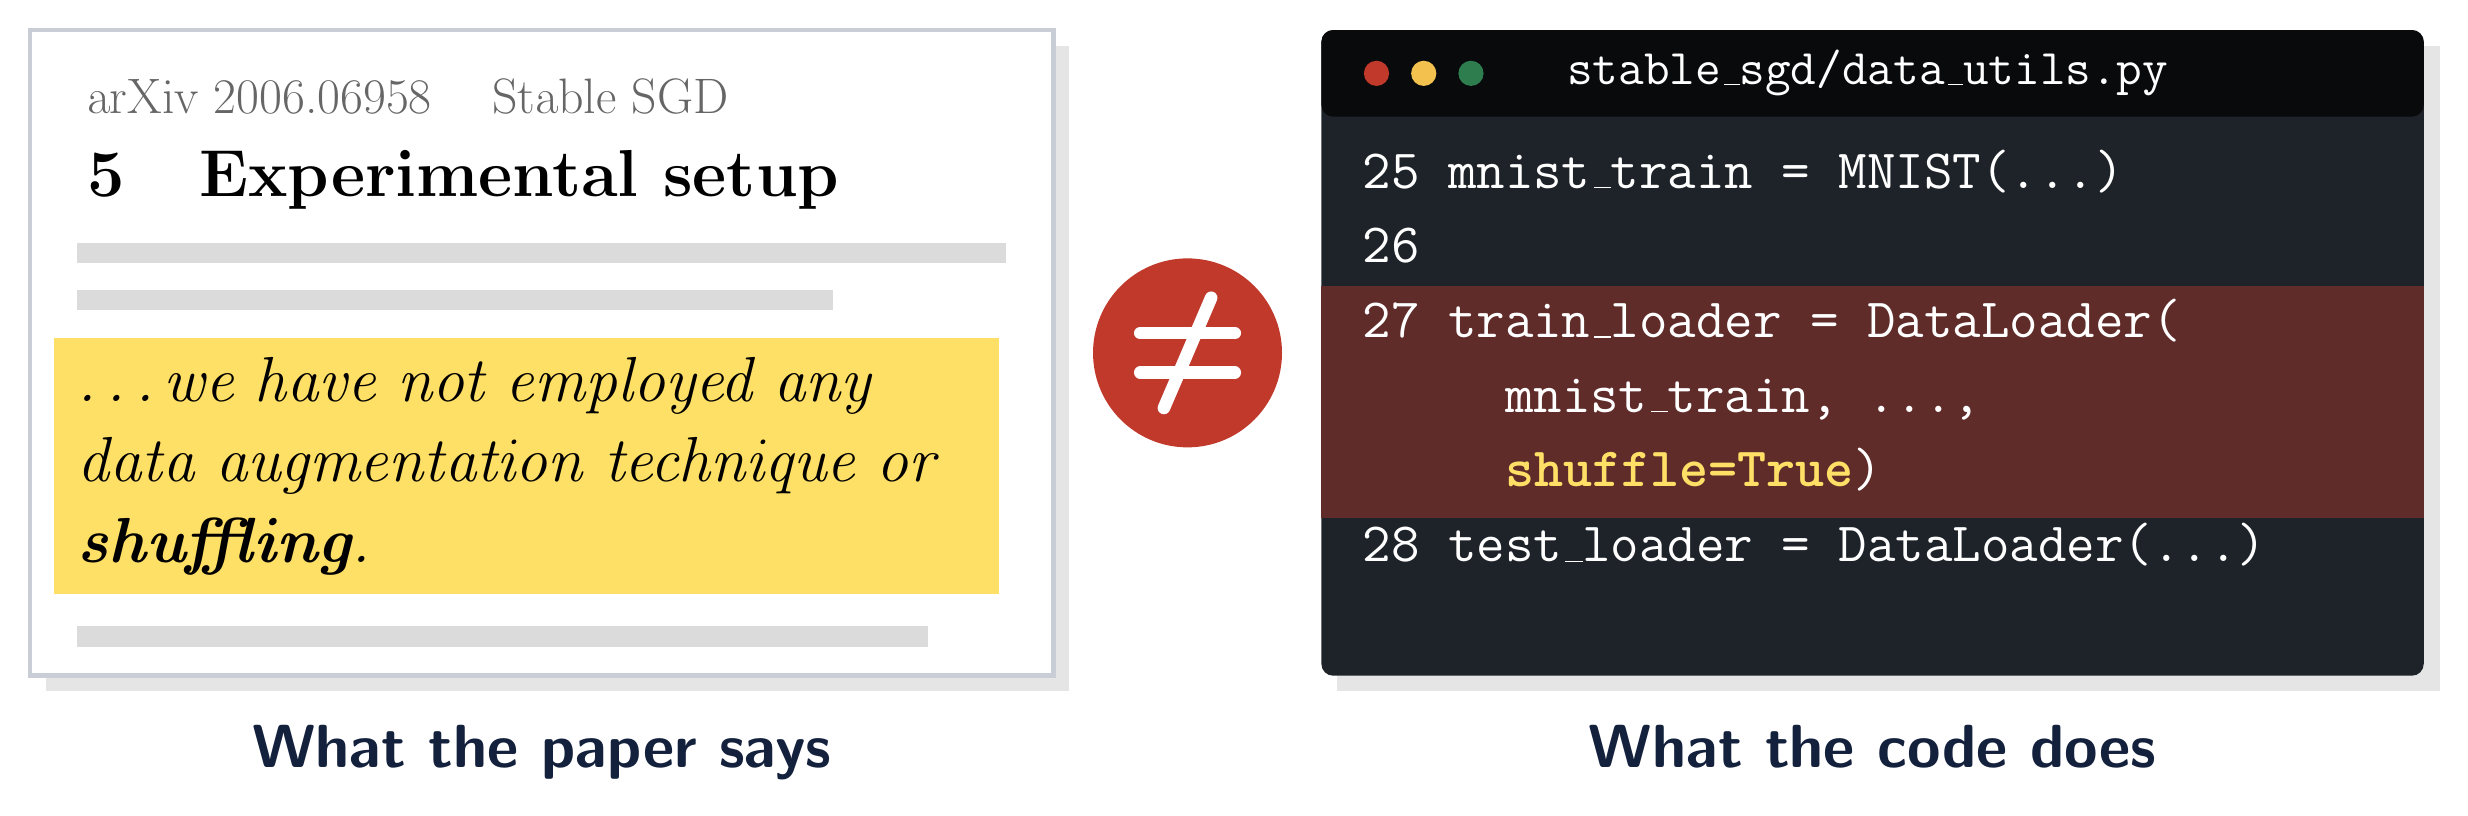
\begin{tikzpicture}[x=1mm,y=1mm]
  % mock paper page
  \fill[black!10] (2,-2) rectangle (132,-84);
  \draw[rulegrey, line width=0.6mm, fill=white] (0,0) rectangle (130,-82);
  \node[anchor=north west, font=\fontsize{18}{22}\selectfont\rmfamily\color{black!60}] at (6,-5) {arXiv 2006.06958 \quad Stable SGD};
  \node[anchor=north west, font=\fontsize{24}{28}\selectfont\rmfamily\bfseries] at (6,-14) {5\quad Experimental setup};
  \foreach \y/\w in {-27/118,-33/96} \fill[black!14] (6,\y) rectangle (6+\w,\y-2.6);
  \node[anchor=north west, fill=hilite, text width=114mm, inner xsep=3mm, inner ysep=2.5mm,
    font=\fontsize{23}{29}\selectfont\rmfamily\itshape] (quote) at (3,-39)
    {\ldots we have not employed any data augmentation technique or \textbf{shuffling}.};
  \fill[black!14] ([yshift=-4mm]quote.south west -| 6,0) rectangle ++(108,-2.6);
  % not-equal badge
  \fill[bad] (147,-41) circle (12);
  \draw[white, line width=1.6mm, line cap=round] (141,-38.5) -- (153,-38.5) (141,-43.5) -- (153,-43.5);
  \draw[white, line width=1.6mm, line cap=round] (144,-48) -- (150,-34);
  % mock code editor
  \fill[black!10] (166,-2) rectangle (306,-84);
  \fill[codebg, rounded corners=1.5mm] (164,0) rectangle (304,-82);
  \fill[black!70!codebg, rounded corners=1.5mm] (164,0) rectangle (304,-11);
  \foreach \i/\c in {0/bad,1/crev,2/good} \fill[\c] (171+\i*6,-5.5) circle (1.6);
  \node[anchor=west, font=\fontsize{18}{22}\selectfont\ttfamily\color{white!80}] at (194,-5.5) {stable\_sgd/data\_utils.py};
  \fill[bad!40!codebg] (164,-32.5) rectangle (304,-62);
  \node[anchor=north west, align=left, font=\fontsize{20}{27}\selectfont\ttfamily\color{white!90}] at (168,-14)
    {{\color{white!45}25}\ mnist\_train = MNIST(\ldots)\\
     {\color{white!45}26}\ \\
     {\color{white!45}27}\ train\_loader = DataLoader(\\
     {\color{white!45}\phantom{27}}\ \ \ mnist\_train, \ldots,\\
     {\color{white!45}\phantom{27}}\ \ \ \textbf{\color{hilite}shuffle=True})\\
     {\color{white!45}28}\ test\_loader = DataLoader(\ldots)};
  \node[anchor=north, font=\fontsize{22}{26}\selectfont\bfseries\color{ink}] at (65,-87) {What the paper says};
  \node[anchor=north, font=\fontsize{22}{26}\selectfont\bfseries\color{ink}] at (234,-87) {What the code does};
\end{tikzpicture}}\par}

\vspace{9mm}
The paper says the data is not shuffled, and the released code shuffles it. \hlmark{We did not plant
this error.} Our auditor found it and quoted both lines.

\vspace{6mm}
ICLR 2027 received \textbf{62,000+} abstracts, far too many to check by hand.
\end{col}\hfill
\begin{col}{0.36\linewidth}{r1}
\sect{Results}
\begin{minipage}[t]{0.5\linewidth}\stat{cfull}{0.636}{Macro-F1}{baselines: 0.05}\end{minipage}%
\begin{minipage}[t]{0.5\linewidth}\stat{good}{0}{false alarms}{on 72 clean items}\end{minipage}

\vspace{14mm}
\begin{minipage}[t]{0.5\linewidth}\stat{blue}{100\%}{flags with a quote}{baselines: 0\%}\end{minipage}%
\begin{minipage}[t]{0.5\linewidth}\stat{ink}{\rs7.4}{per paper}{B1 (Agent): \rs51}\end{minipage}

\vspace{14mm}
{\smalltext\color{black!70} Tested on 40 papers with their code, plus a copy of each with planted errors (163 errors).\par}
\end{col}

\vspace{6mm}

% ================================================================ row 2: how it works | web app
\begin{col}{0.77\linewidth}{r2}
\sect{\raisebox{-0.18em}{
\includegraphics[height=1.15em]{../logo.png}}\hspace{0.3em}Our system}
You give the auditor a paper (PDF or LaTeX) and its code. It checks every reference, citation,
stated setting and claim against the cited paper or the code, and \textbf{reports a problem only
when it can quote both sides}.

\vspace{4mm}
\resizebox{\linewidth}{!}{%
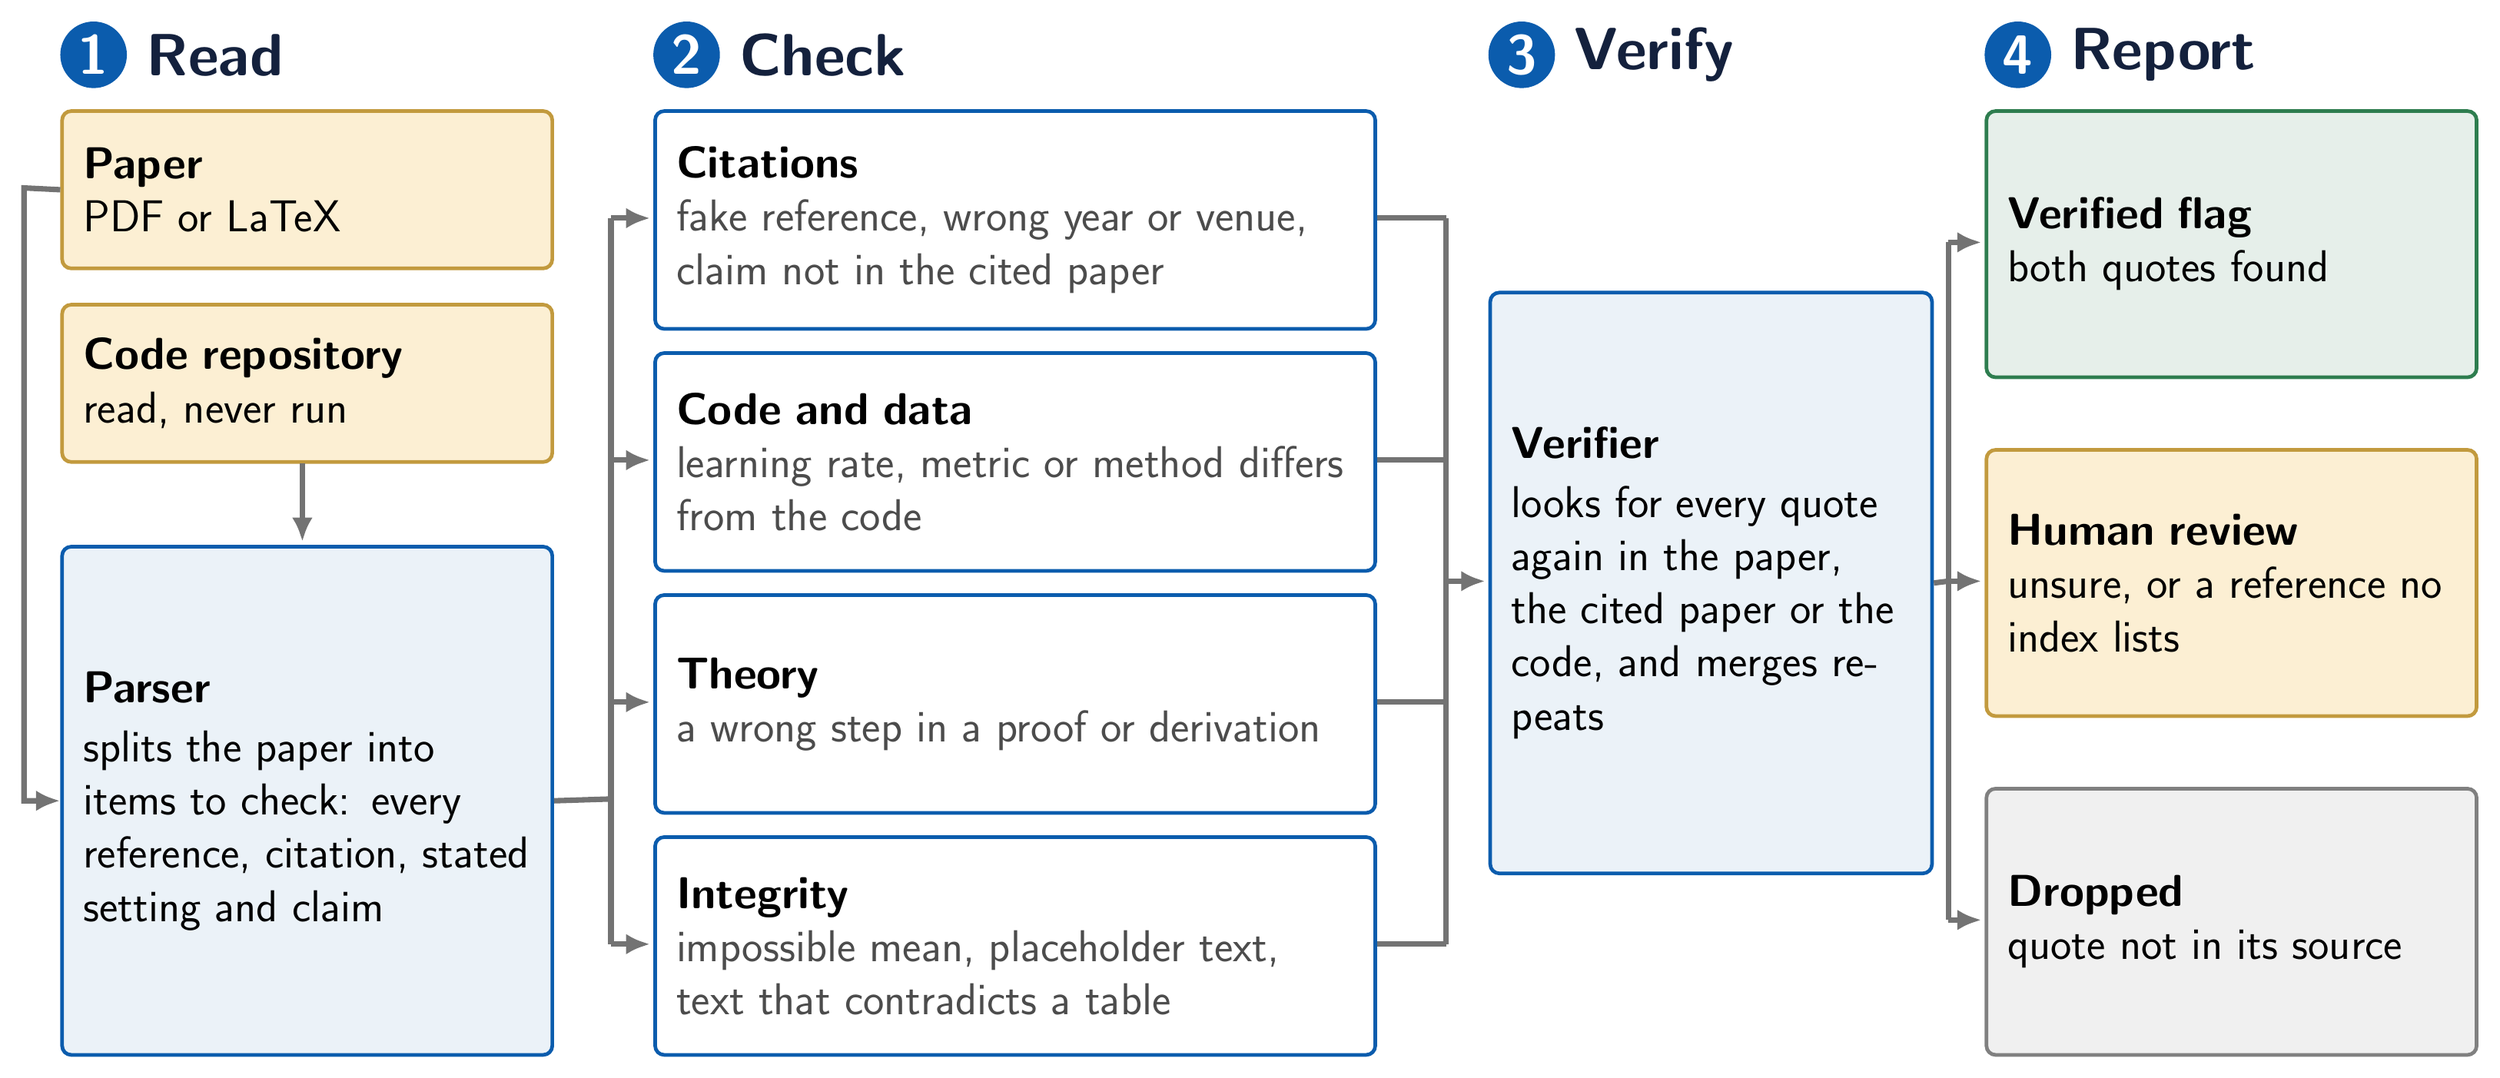
\begin{tikzpicture}[x=1mm, y=1mm, font=\sffamily\fontsize{21}{25}\selectfont,
  bx/.style={draw=#1, line width=0.6mm, rounded corners=1.5mm, align=left, inner xsep=3.5mm,
    inner ysep=2mm, anchor=north west},
  ar/.style={-{Latex[length=4mm,width=3.4mm]}, line width=0.9mm, black!55},
  ln/.style={line width=0.9mm, black!55},
  stepno/.style={circle, fill=blue, text=white, minimum size=11mm, inner sep=0pt,
    font=\sffamily\bfseries\fontsize{26}{26}\selectfont},
  stitle/.style={anchor=west, font=\sffamily\bfseries\fontsize{28}{32}\selectfont\color{ink}}]
% ---- stage titles
\foreach \x/\n/\s in {0/1/Read, 98/2/Check, 236/3/Verify, 318/4/Report} {
  \node[stepno] at (\x+5.5,9) {\n};
  \node[stitle] at (\x+13,9) {\s};
}
% ---- 1 read
\node[bx=crev!80!black, fill=crev!25, text width=74mm, minimum height=26mm] (pdf) at (0,0)
  {\textbf{Paper}\\ PDF or LaTeX};
\node[bx=crev!80!black, fill=crev!25, text width=74mm, minimum height=26mm] (repo) at (0,-32)
  {\textbf{Code repository}\\ read, never run};
\node[bx=blue, fill=blue!8, text width=74mm, minimum height=84mm] (parse) at (0,-72)
  {\textbf{Parser}\\[1mm] splits the paper into items to check: every reference, citation,
   stated setting and claim};
\draw[ar] (40,-58.5) -- (40,-71.5);
\draw[ar] (pdf.west) -- (-6,-13) |- (parse.west);
% ---- 2 check
\foreach \y/\name/\what [count=\i] in {
   0/Citations/{fake reference, wrong year or venue, claim not in the cited paper},
  -40/Code and data/{learning rate, metric or method differs from the code},
  -80/Theory/{a wrong step in a proof or derivation},
  -120/Integrity/{impossible mean, placeholder text, text that contradicts a table}} {
  \node[bx=blue, fill=white, text width=112mm, minimum height=36mm] (c\i) at (98,\y)
    {\textbf{\name}\\ {\color{black!70}\what}};
}
\draw[ln] (parse.east) -- (91,-114);
\draw[ln] (91,-18) -- (91,-138);
\foreach \y in {-18,-58,-98,-138} \draw[ar] (91,\y) -- (97.5,\y);
% ---- 3 verify
\foreach \i/\y in {1/-18, 2/-58, 3/-98, 4/-138} \draw[ln] (c\i.east |- 0,\y) -- (229,\y);
\draw[ln] (229,-18) -- (229,-138);
\node[bx=blue, fill=blue!8, text width=66mm, minimum height=96mm] (ver) at (236,-30)
  {\textbf{Verifier}\\[1mm] looks for every quote again in the paper, the cited paper or the
   code, and merges repeats};
\draw[ar] (229,-78) -- (235.5,-78);
% ---- 4 report
\node[bx=good, fill=good!12, text width=74mm, minimum height=44mm] (ok) at (318,0)
  {\textbf{Verified flag}\\ both quotes found};
\node[bx=crev!80!black, fill=crev!25, text width=74mm, minimum height=44mm] (hum) at (318,-56)
  {\textbf{Human review}\\ unsure, or a reference no index lists};
\node[bx=black!50, fill=black!6, text width=74mm, minimum height=44mm] (drop) at (318,-112)
  {\textbf{Dropped}\\ quote not in its source};
\draw[ln] (ver.east) -- (312,-78);
\draw[ln] (312,-22) -- (312,-134);
\foreach \y in {-22,-78,-134} \draw[ar] (312,\y) -- (317.5,\y);
\end{tikzpicture}}
\end{col}\hfill
\begin{col}{0.215\linewidth}{r2}
\sect{The web app}
\setlength{\fboxsep}{0pt}\setlength{\fboxrule}{0.6mm}\centering
\fcolorbox{rulegrey}{white}{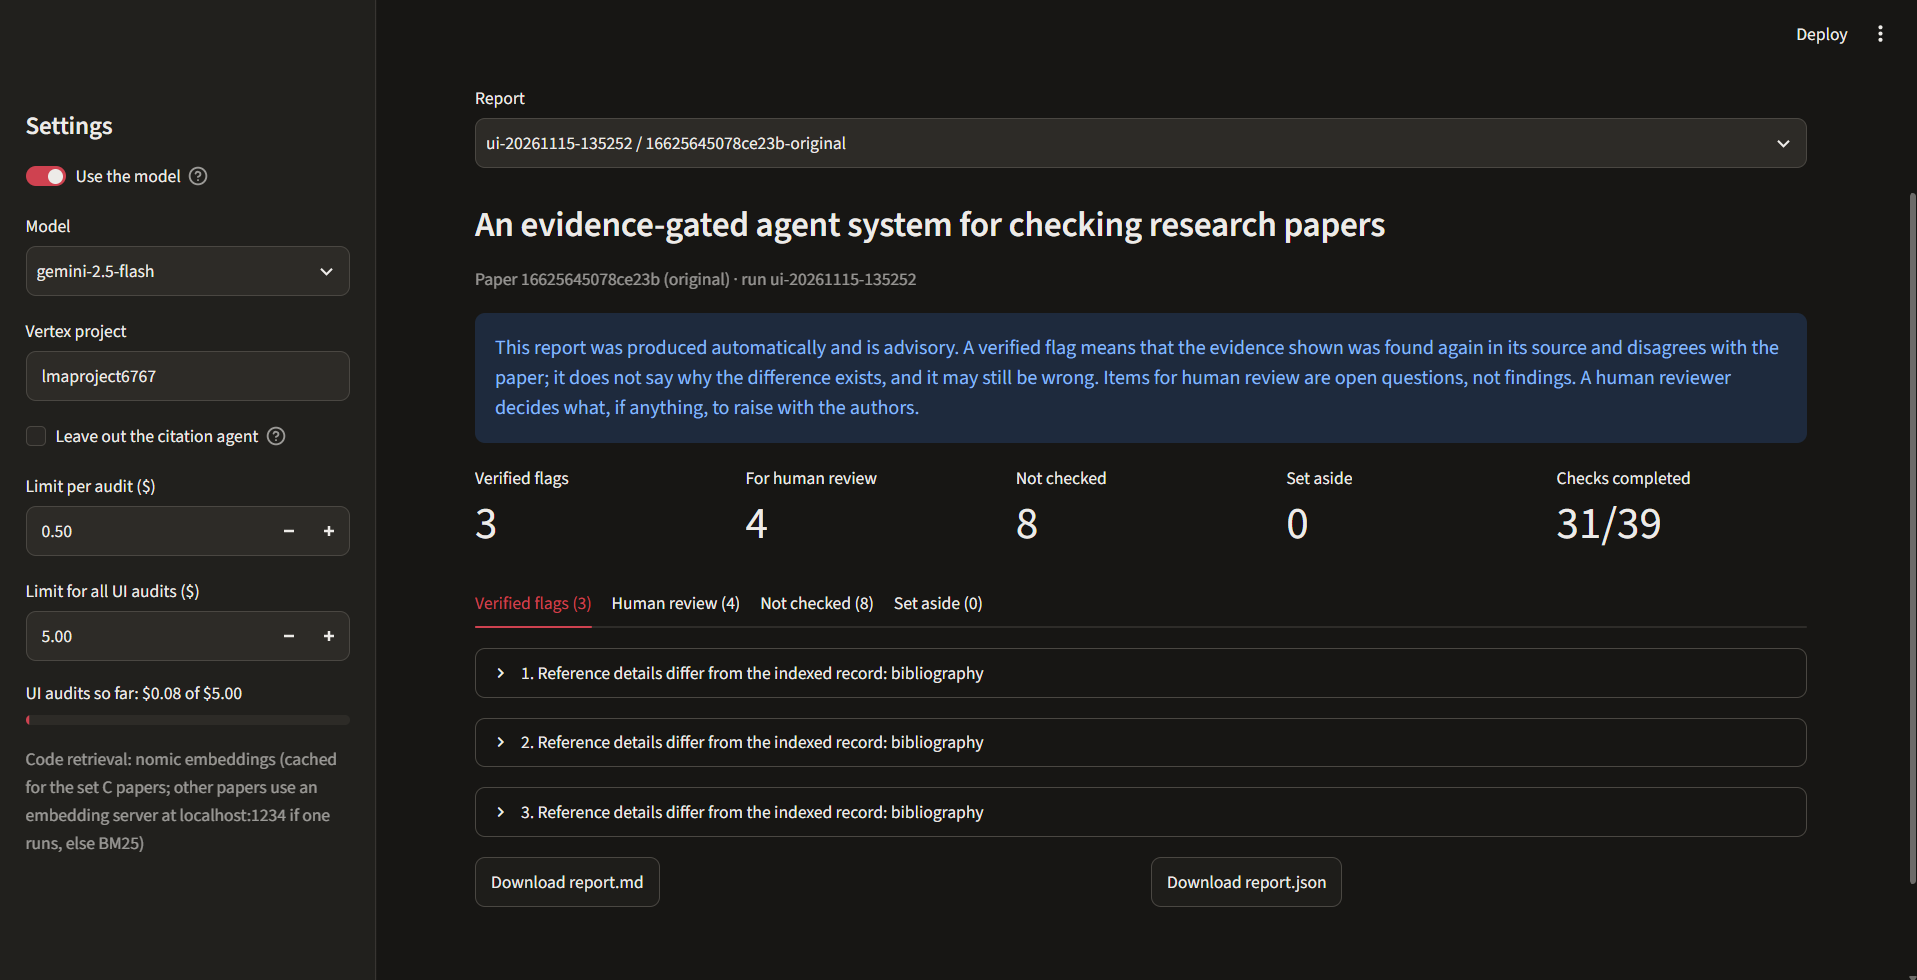
\includegraphics[width=\dimexpr\linewidth-1.2mm\relax, trim=273 48 58 60, clip]{../app_screenshots/report_result.png}}\\[3mm]
{\smalltext Results by outcome}\\[6mm]
\fcolorbox{rulegrey}{white}{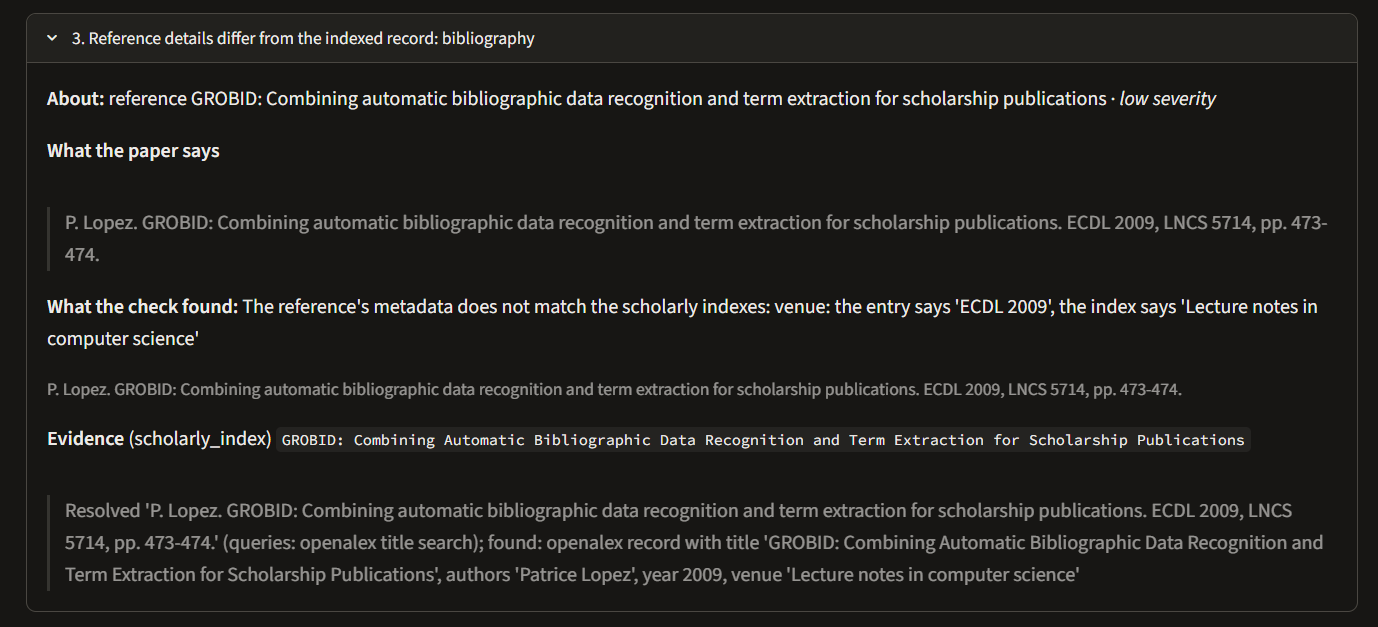
\includegraphics[width=\dimexpr\linewidth-1.2mm\relax]{../app_screenshots/detailed_claim.png}}\\[3mm]
{\smalltext One flag with its evidence}
\end{col}

\vspace{6mm}

% ================================================================ row 3: three results
\begin{col}{0.335\linewidth}{r3}
\sect{Finds what an LLM misses}
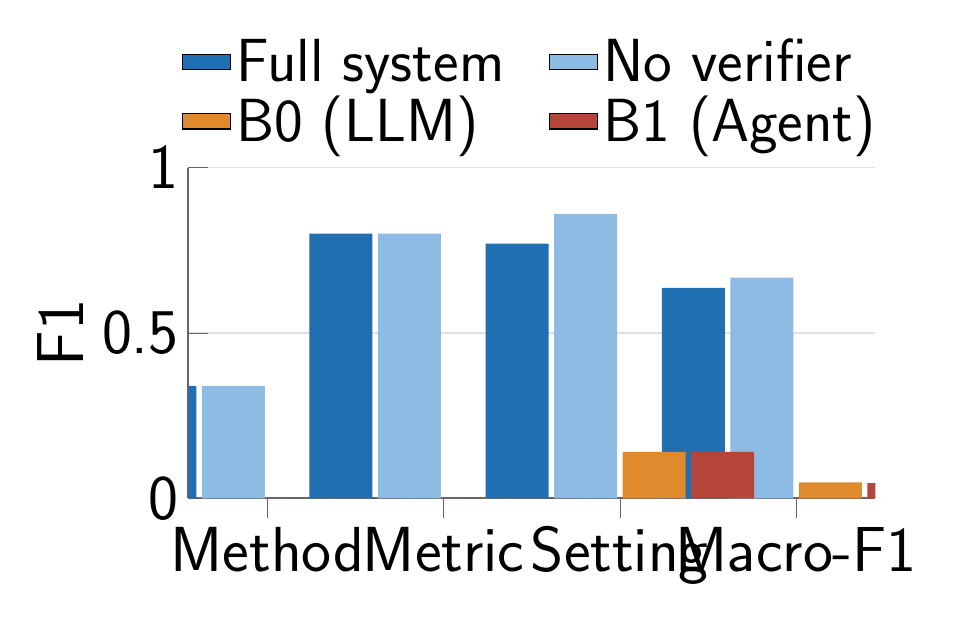
\begin{tikzpicture}
\begin{axis}[poster, width=\linewidth-34mm, height=42mm, scale only axis,
  ybar, bar width=8mm, ymin=0, ymax=1, area legend,
  symbolic x coords={Method,Metric,Setting,Macro-F1}, xtick=data,
  enlarge x limits=0.15, ytick={0,0.5,1}, ylabel={F1},
  legend style={at={(0.5,1.03)}, anchor=south, legend columns=2, draw=none, fill=none,
    font=\fontsize{22}{27}\selectfont, cells={anchor=west},
    /tikz/every even column/.append style={column sep=5mm}},
  ymajorgrids, axis x line*=bottom, axis y line*=left]
\addplot[fill=cfull,draw=none] coordinates {(Method,0.34) (Metric,0.80) (Setting,0.77) (Macro-F1,0.636)};
\addplot[fill=cnover,draw=none] coordinates {(Method,0.34) (Metric,0.80) (Setting,0.86) (Macro-F1,0.667)};
\addplot[fill=cbzero,draw=none] coordinates {(Method,0) (Metric,0) (Setting,0.14) (Macro-F1,0.048)};
\addplot[fill=cbone,draw=none] coordinates {(Method,0) (Metric,0) (Setting,0.14) (Macro-F1,0.046)};
\legend{Full system, No verifier, B0 (LLM), B1 (Agent)}
\end{axis}
\end{tikzpicture}

\vspace{7mm}
We aimed for 10 points of Macro-F1 above the baselines and got \hlmark{59.}

\vspace{4mm}
{\smalltext Neither baseline finds a method or metric error. On its own, the citation checker scores \textbf{F1 0.879} on HALLMARK.\par}
\end{col}\hfill
\begin{col}{0.315\linewidth}{r3}
\sect{Better and cheaper}
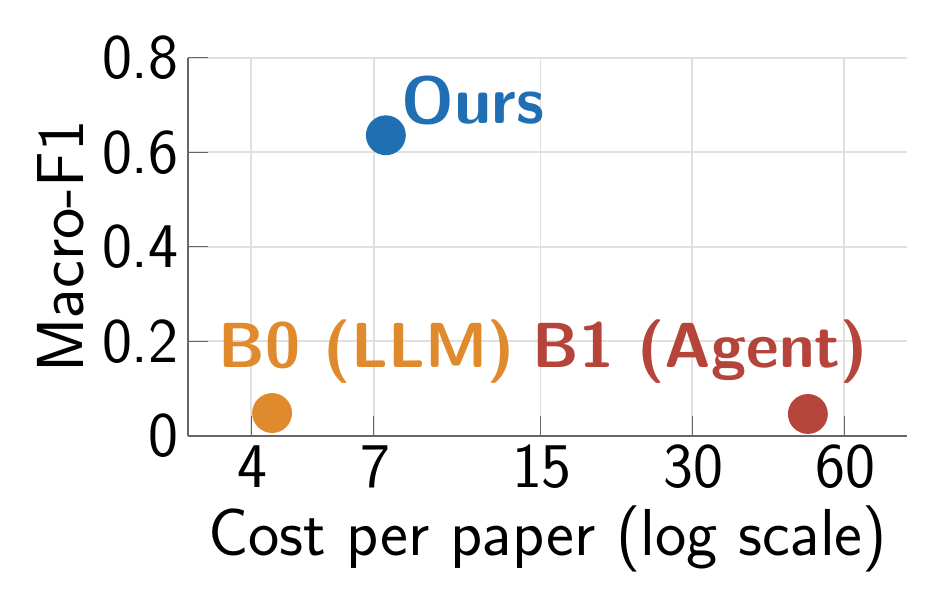
\begin{tikzpicture}
\begin{semilogxaxis}[poster, width=\linewidth-30mm, height=48mm, scale only axis,
  xmin=3, xmax=80, ymin=0, ymax=0.8,
  xtick={4,7,15,30,60}, xticklabels={\rs4,\rs7,\rs15,\rs30,\rs60},
  ytick={0,0.2,0.4,0.6,0.8},
  xlabel={Cost per paper (log scale)}, ylabel={Macro-F1},
  grid=major, axis x line*=bottom, axis y line*=left]
\addplot[only marks, mark=*, mark size=7pt, cfull] coordinates {(7.4,0.636)};
\addplot[only marks, mark=*, mark size=7pt, cbzero] coordinates {(4.4,0.048)};
\addplot[only marks, mark=*, mark size=7pt, cbone] coordinates {(50.9,0.046)};
\node[anchor=south west, font=\fontsize{24}{28}\selectfont\bfseries\color{cfull}] at (axis cs:7.6,0.64) {Ours};
\node[anchor=south west, font=\fontsize{23}{27}\selectfont\bfseries\color{cbzero}] at (axis cs:3.3,0.09) {B0 (LLM)};
\node[anchor=south east, font=\fontsize{23}{27}\selectfont\bfseries\color{cbone}] at (axis cs:70,0.09) {B1 (Agent)};
\end{semilogxaxis}
\end{tikzpicture}

\vspace{7mm}
Ours costs \textbf{\rs7.4} a paper and B1 (Agent) costs \hlmark{\rs51.}

\vspace{4mm}
{\smalltext B1 sends the whole paper with each of its 20 calls. Converted at \rs94 per US\$.\par}
\end{col}\hfill
\begin{col}{0.32\linewidth}{r3}
\sect{Fewer flags to check}
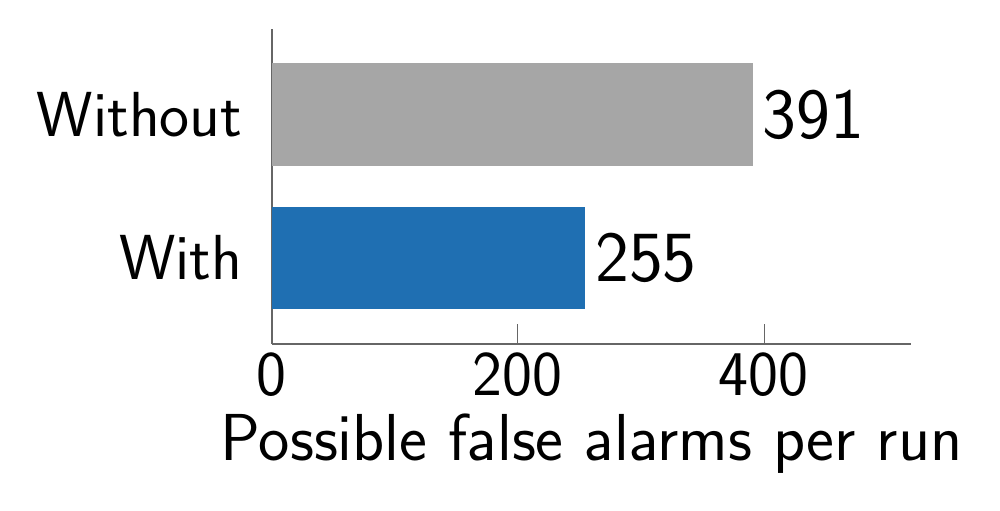
\begin{tikzpicture}
\begin{axis}[poster, width=\linewidth-40mm, height=40mm, scale only axis,
  xbar, bar width=13mm, bar shift=0pt, xmin=0, xmax=520, ytick={1,2}, yticklabels={With,Without},
  ymin=0.4, ymax=2.6, xtick={0,200,400},
  xlabel={Possible false alarms per run}, axis x line*=bottom, axis y line*=left, ytick style={draw=none},
  nodes near coords, every node near coord/.append style={anchor=west, font=\sffamily\fontsize{26}{30}\selectfont\bfseries}]
\addplot[fill=cfull,draw=none] coordinates {(255,1)};
\addplot[fill=black!35,draw=none] coordinates {(391,2)};
\end{axis}
\end{tikzpicture}

\vspace{7mm}
With the verifier, a reviewer has \hlmark{35\% fewer} flags to check.

\vspace{4mm}
{\smalltext Of the 203 planted errors found, 180 were verified and 23 went to a human. The verifier costs 3 points of F1.\par}
\end{col}

\vspace{6mm}
\begin{minipage}[c]{0.6\linewidth}
  {\fontsize{32}{40}\selectfont\bfseries\color{ink} CL3.410 LMA \quad$\cdot$\quad final project}
\end{minipage}\hfill
\begin{minipage}[c]{0.38\linewidth}\raggedleft
  {\fontsize{24}{28}\selectfont\bfseries\color{ink}\faGithub\ Code}\enspace
  \raisebox{-0.5\height}{\qrcode[height=24mm]{\codeurl}}\hspace{12mm}%
  {\fontsize{24}{28}\selectfont\bfseries\color{ink}\faGlobe\ Website}\enspace
  \raisebox{-0.5\height}{\qrcode[height=24mm]{\websiteurl}}
\end{minipage}

\end{document}
